\documentclass[a4paper,10pt]{article}
%
\usepackage{amsmath}
\usepackage{amssymb}
\usepackage{amstext}
\usepackage[bookmarks,colorlinks]{hyperref}
\usepackage{makeidx}
\usepackage{graphicx}
\makeindex
%
%--------------------   start of the 'preamble'
%
%%    homebrew commands -- to save typing
\newcommand\etc{\textsl{etc}}
\newcommand\eg{\textsl{eg.}\ }
\newcommand\etal{\textsl{et al.}}
\newcommand\Quote[1]{\lq\textsl{#1}\rq}
\newcommand\fr[2]{{\textstyle\frac{#1}{#2}}}
\newcommand\miktex{\textsl{MikTeX}}
\newcommand\comp{\textsl{The Companion}}
\newcommand\nss{\textsl{Not so Short}}
%
%---------------------   end of the 'preamble'
%
\begin{document}
%-----------------------------------------------------------
\title{Technical Report of iZENELib}
\author{Yingfeng Zhang, Kevin Hu}
\maketitle
%--------------------------------------------------
\begin{abstract}\centering
  This document presents the technical report for the project \emph{iZENELib} that could be used in the search engine developing process.
\emph{iZENELib} is expected to contain two parts:AM-Lib, which takes charge of storage, and IR-Lib, which takes charge of information 
retrieval and machine learning.
\end{abstract}
%--------------------------------------------------

%--------------------------------------------------
\tableofcontents
%--------------------------------------------------

\section{Document History}
\begin{tabular}{|c|c|p{7cm}|}
    \hline
    Date & Author & Description \\ \hline
    2008-11-02& Kevin & Initialize the design issue of AM-Lib. \\ \hline
    2008-11-10& Yingfeng & Initialize the design issue of IR-Lib.  \\ \hline
    2008-11-10& Yingfeng & Create the technical report.  \\ \hline
\end{tabular}

\section{Design Goal}
 \emph{iZENELib} plans to provide a collection of utilities which could be used in the search engine developing process.
\emph{iZENELib} is expected to be composed of two parts---the part taking charge of storage(AM-Lib), and the part in charge
of information retrieval and machine learning(IR-Lib). AM-Lib is expected to be composed of two sub-parts, the one which provides 
common utilities for data storage, and the one providing corpus data management which serves for the IR-Lib. Generic design would 
be adopted largely in \emph{iZENELib} to provide much more flexibility for component's reusing.

\section{Initial architecture design of AM-lib}
The future probable usages of AM-lib can be illustrated in several ways.
\begin{itemize}
 \item[$\bullet$] In your project, you may want to compare the performance of using several different data structures. AM-lib makes this easy anyway.

\begin{scriptsize}\begin{verbatim}
                #include "am/am.hpp''
                class MyClass {

                public: 
                        MyClass(AccessMethods<int, string>* pAm): pAm_(pAm){}

                        void myFoo()
                        {
                                pAm_->insert(128, ``Hello! AM-lib``);
                                pAm_->getDataBy(128);
                                . . .
                        }

                private:
                        AccessMethods<int, string>* pAm_;
                }

                ////////////////////////////////////
                #include "myclass.hpp''
                #include "am/btree.hpp''
                #include "am/rtree.hpp''
                #include "am/am.hpp''
                int main()
                {
                        AccessMethods<int, string>* pAm = new BTree<int, string>(...);
                        MyClass test1(pAm);
                        test1.myFoo();
                        delete pAm;
                        . . .
                        pAm = new RTree<int, string>(...);
                        MyClass test2(pAm);
                        test2.myFoo();
                        delete pAm;
                        . . .
                }
\end{verbatim}                \end{scriptsize}

 \item[$\bullet$] You can make your modules more reuseable.
\begin{scriptsize}\begin{verbatim}
                template<typename AmType>
                void foo(AmType& am)
                {
                        am.insert(128, ``Hello! AM-lib``);
                        am.getDataBy(128);
                }

                ////////////////////////////////////
                #include "am/btree.hpp''
                #include "am/rtree.hpp''
                int main()
                {
                        BTree<int, string> btree;
                        foo(btree);
                        . . .
                        RTree<int, string> btree;
                        foo(btree);
                        . . .
                }
\end{verbatim}                \end{scriptsize}

\item[$\bullet$] You don't need to worry about the size of data, cause AM-lib will use disk when data size comes very large.
\begin{scriptsize}\begin{verbatim}
                void foo(AmType& am)
                {
			//initialize a 3 dimensions dynamic array
                        MulDimDynArray largeArray(100000000, 100000000, 1000000);
                        MulDimDynArray smallArray(10, 10, 10);
                        smallArray.append(largeArray);
                        . . .
                }
\end{verbatim}                \end{scriptsize}

\end{itemize}

\par
\begin{figure}[h!]
\centerline{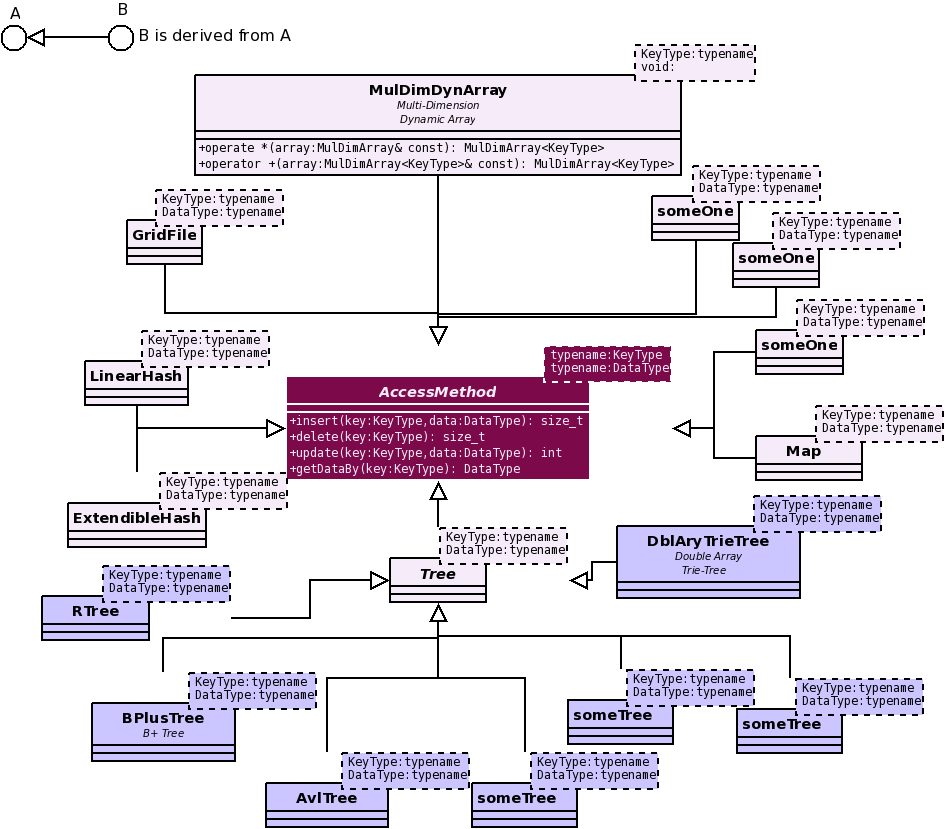
\includegraphics[width=\textwidth]{architecture.png}}
\caption{Initial design of AM-lib classes}\label{architecture}
\end{figure}

\begin{figure}[ht]\centering
  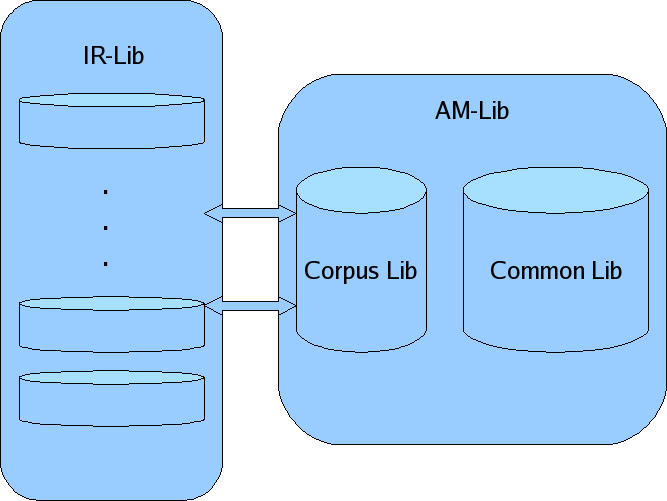
\includegraphics[width=.7\textwidth]{fig1.png}
  \caption{AM-Lib and IR-LIB}\label{fig:pic}
\end{figure}

\section{Corpus Management}
Corpus management component of AM-Lib provides storage services for IR-Lib. It is necessary because each component of 
IR-Lib will read data from corpus and output the results to a generic structs, therefore refactoring this common part into a 
single library will improve the system's reusage.
\par
Existing project as \emph{SML} provides similiar components as \textsc{DocumentBag},etc. We can base corpus management on
\textsc{sml}. What's more, IR-Lib needs a powerful matrix component to store the middle temporary computation outputs and 
the ultimate results. Through research, such a matrix component is expected to be included in \emph{iZENELib}:

\label{sec:notation}

\begin{itemize}
\item A general matrix that has both memory and file version.

  Memory version of matrix has been provided by \emph{Boost}, and file version has been implemented by \emph{Clustering-framework}.
Therefore it is necessary to provide the general matrix with an improvement on them.

\item SVD Decomposition, QR Decomposition, LU Decomposition, Eigenvalue Decomposition.

 These utilities are extremly useful in machine learning and information retrieval.

\item Hessian matrix 

 Hessian matrix is useful in Bayesian inference and decision theory.
\end{itemize}
 \par
During the developing process of \emph{iZENELib}, more components of matrix would perhaps be included if necessary.

\section{Components of IR-Lib}
\label{sec:fwv}
IR-Lib is a collection of algorithms in machine learning and information retrieval, together with the Corpus Management component of 
AM-Lib, it could provide a generic framework for search applications. Both machine learning and information retrieval have covered lots
of fields, therefore, the main purpose of IR-Lib is to provide a scalable framework together with general algorithms, then in future, more
advanced algorithms could be added easily.
\par
The relationship between machine learning and information retrieval is very close and machine learning could be seen as the lower layer to
provide methods for information retrieval's usage. Therefore IR-Lib could be composed of two layers. In addition, there exists some fields
in information retrieval that has not adopted methods provided by machine learning, such as recommendation systems, preprocessing, etc. We
will talk about all the components of IR-Lib one by one.

\section{Machine learning Components}
\begin{itemize}
  \item Supervised Learning.\\
\emph{Wisenut-classifier} has implemented most of the basic supervised learning methods. We plan to replace the interface to \emph{SML}
 with the interface to new corpus management component of AM-Lib, and then refactor it to the generic design.
  \item Unsupervised Learning.\\
\emph{Clustering-framework} has already doen a good job of it. Therefore, the relavant job of this component is to make \emph{Clustering-framework}
suit for the whole framework of IR-Lib.
  \item Learning Complex Models.
    \begin{enumerate}
	\item EM(Expectation---Maximization), which is also a basic learning approach in semi-supervised learning.
	\item Hidden Markov Models.
	\item Sampling method, including MCMC.
	\item Graphical Models, graphical models including following directions, each of which is under hot research, we are not sure whether 
it is possible to implement all of them, just try to do that.
          \begin{enumerate}
            \item Bayesian Network.
            \item Markov Random Fields.
            \item Conditional Random Fields.
          \end{enumerate}
    \end{enumerate}
  \item Dimensionality Reduction. We plan to implement PCA at first, more approaches could be done in future if possible.
\end{itemize}
\par
In summary, machine learning are still under fast developing process, therefore only some basic directions would be included into this library, we hope a 
good design framework could be provided in order that more learning approaches could be included into this library easily in future.

\section{Information Retrieval Components}
\begin{itemize}
 \item Text Pre-Processing\\
Text pre-processing techniques are mature and have been implemented by existing projects, therefore we can refactor them from existing code.
    \begin{enumerate}
     \item Stopword Removal
     \item Stemming
     \item TF-IDF
     \item Tokenization
     \item Feature Selection
     \item Duplicate Detection
    \end{enumerate}
  \item Language Models\\
It is necessary to refactor and integrate Jinglei's work into the library.
  \item Topic Modeling\\
Topic modelling is a hot research direction and lots of new approaches appear continuously. We only plan to provide some topic modelling methods including
LSI, LDA and 4-level PAM. We hope more topic modeling approaches could be easily added to this library.
\end{itemize}

\section{Schedule}
Kevin and I will take main charge of implemeting \emph{iZENELib}, however, since both of us have other projects to maintain and therefore we could not 
guarantee the certian time to finish this project. We hope to finish it before Spring Festival at the end of Jan,2009.\\
\par
\centering
\begin{tabular}{|p{3cm}|c|c|p{4cm}|}
    \hline
    MileStone & Finish Date & In Charge & Description \\ \hline
    AM-Lib& 2008-12-15 & Kevin & AM-Lib has been finished \\ \hline
    Basic IR-Lib& 2008-12-15 & Yingfeng & Basic IR-Lib could be provided, including corpus management, basic supervised and unsupervised learning.  \\ \hline
    Pre-Processing& 2008-12-31 & Kevin & Text pre-processing component is encapsulated.  \\ \hline
    Complex machine learning& 2009-01-15 & Yingfeng & Learning methods for complex models have been finished. \\ \hline
    Language models and topic models& 2009-01-31 & Yingfeng & Finish IR-Lib. \\ \hline
\end{tabular}

\end{document}